\section{Experiment}

\subsection{Procedure}
 In the experiment 4,351 participants had to fill out custom demographic questions on the Lucid website. In order to qualify, the participant had to satisfy all of the following criteria: brought up monolingually, hold nationality of the country we targeted, speak the language as a native and use it as their first language.

In the first page the participants are presented with a consent page. Here they accept the conditions of privacy and data collection. The first part of the experiment is Wikivocab (See Sec. \ref{wikivocab}), a pre-screener test to determine the participant's proficiency of the examined language. Subsequently, the participants had to pass the main experiment. Here they were presented with a color square (See Sec. \ref{stimuli}) which they had to name with a basic color term (See Sec. \ref{paradigm}). After completion of all trials, the participants where forwarded to a color blindness test (See Sec.\ref{col-blindness}). At the end of the experiment, the participants were asked about the duration of any training in music and art related activities.

\subsection{Software Implementation}
The Experiment was implemented using Psynet \footnote{\url{https://www.psynet.dev}}. Psynet is a framework built on Dallinger which is a platform to host and deploy online experiments \footnote{\url{https://github.com/Dallinger/Dallinger}}. It allows you to develop and design complex experiments \parencite{harrisonGibbs2020}. We recruited participants from two different crowd-sourcing platforms: Prolific \parencite{prolific} and Lucid platform by Cint \parencite{lucid,cint}. \textcite{lucid} is a platform for recruiting human participants serving as an exchange to connect survey providers and recruting services, which was acquired by the major recruiting firm Cint (\cite{cint}) in 2022. Currently, Cint offers Lucid as one of its services. In this thesis, we refer to the platform as `Lucid' to distinguish the participant group it provides, which may vary from the broader pool available through Cint. The attendees interact with the study via a user interface in their browser. This interface connects to a Python EC2 Server (Amazon Elastic Compute Cloud) cluster on the back end, overseeing the experiment's progression. Additionally, there's a secure Postgres database set up for storing data. To keep the interaction and loading time for the participants low, EC2 servers were provisioned at locations close to the participants location. The availability of the code detailing the experiments is specified in section \ref{code_availability}.

\begin{figure}[htp]
    \centering
    
\includegraphics[width=\textwidth]{psynet-workflow.pdf}
    \decoRule
    \caption[Structure of the data collection infrastructure]{Structure of the data collection infrastructure: Reproduced from Harrison et al., 2020 and updated with more recent deployment platforms Prolific and Lucid.}
    \label{fig:psynet-workflow}
\end{figure}

To counter the arguments that online experiments have a lack of control over the experimental conditions and that participants respond honestly, Psynet offers a range of pre-screen test such as Wikivocab and a color-blindness test.


\subsection{Wikivocab}
\label{wikivocab}
Wikivocab is a pre screen test developed by \textcite{vanrijnWorld2023} to predict the proficiency of participants in languages. It was shown that the test is reliable and can distinguish speaker of closely related languages. The procedure is still under development. By the time we conducted the experiments it supported 36 languages covering all examined languages except Thai. For this test low frequency words are sampled from the Wikipedia corpus as real words. Second, pseudo words are created using an algorithm that preserves the phonotactic structure of the language. The participants are then asked to identify the real words. The test is designed to be language independent and is therefore suitable for a each specific language (Fig. \ref{fig:pre-screens} B).


\subsection{Color Blindness Test}
\label{col-blindness}
The color blindness test of the Psynet framework adapts to the procedure of the Ishihara-color-blindness test \parencite{clark1924ishihara}. An image shows circles of diverging size. Some of these circles are colored such that their connected overall picture shapes a number. Importantly, the used colors and contrasts are designed such that for participant suffering from color perception deficiencies it is hard to distinguish between background and number. Each participant was presented with six trials and had to give at least four correct answers. Participants with a smaller score where excluded from the analysis.
(Fig. \ref{fig:pre-screens} A)

\begin{figure}[htp]
    \centering
    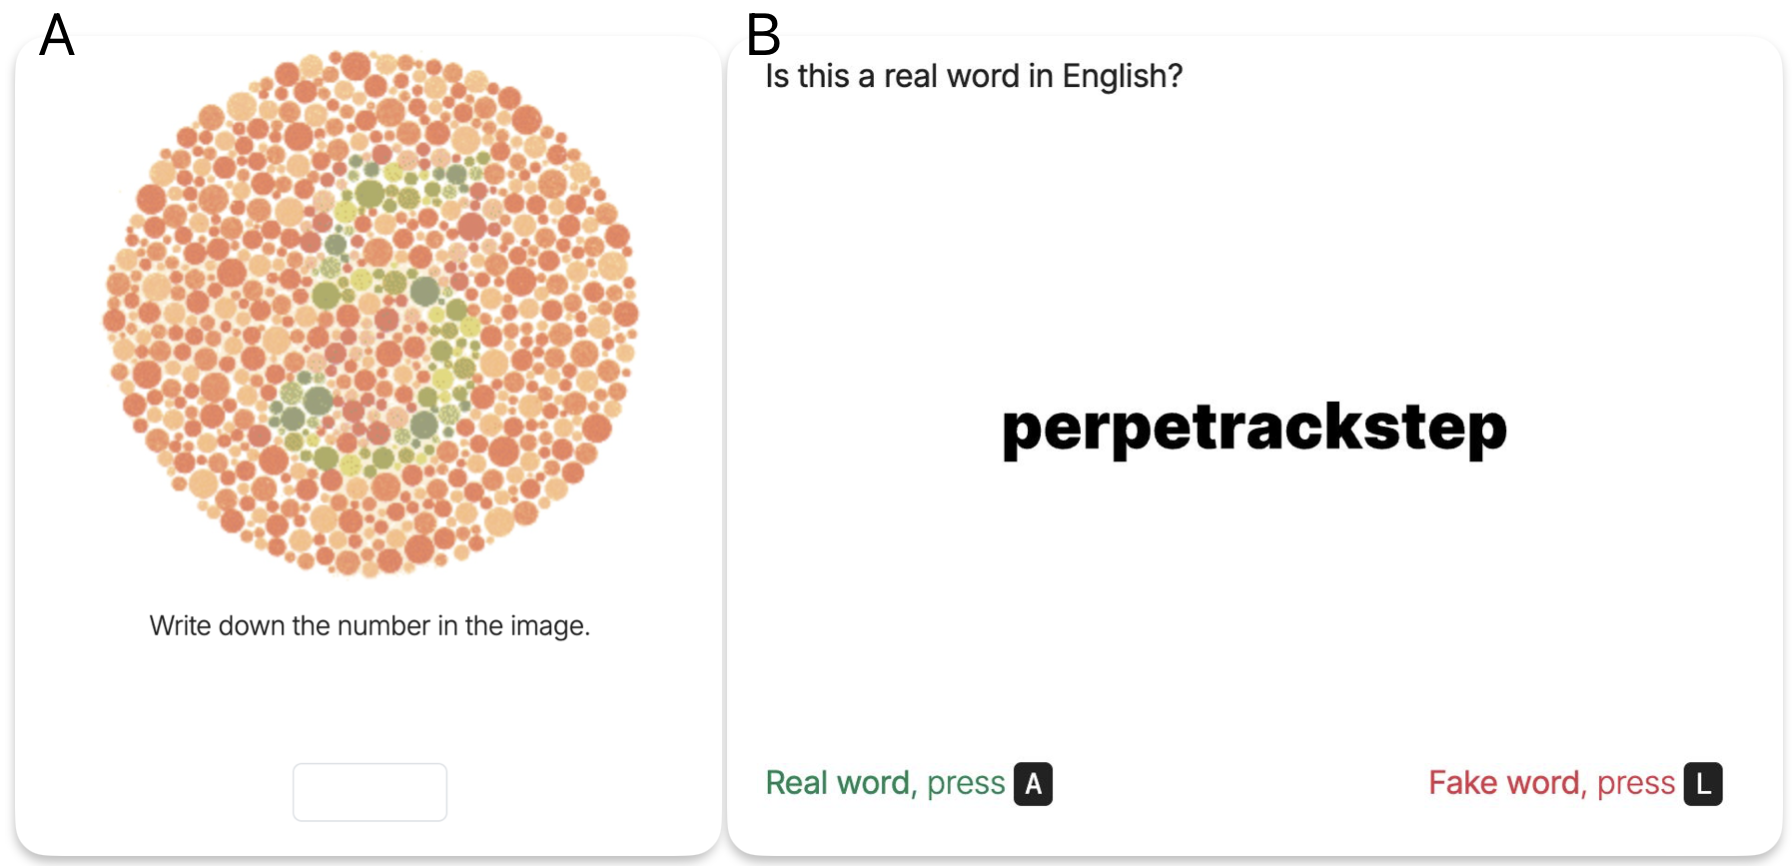
\includegraphics[width=\textwidth]{images/PrescreenTests.png}
    \decoRule
    \caption[Ishihara Color Blindness Test and Wikivocab]{Ishihara Color Blindness Test and Wikivocab: A: Color blindness test adapted to the Ishihara procedure asking participants to report the depicted number. B: Wikivocab trail showing a generated pseudo-word. Participants were to detect real and artificial words.}
    \label{fig:pre-screens}
\end{figure}



\subsection{Paradigm}
\label{paradigm}
There have been multiple paradigms applied in the field of color categorization such as color discrimination \parencite{winawerRussian2007}, serial reproduction \parencite{xuCultural2013}, and similarity judgments \parencite{marjieh2023words}. This study aimed to collect comprehensive up to date color lexicony of a large number of languages. Therefore, we decided to adapt to the free naming task of the World Color Survey \parencite{kayWorld2009}. Participants were asked to freely name presented color patches.

To prevent fatigue, each participant was only presented with a subset of 50 color chips instead of the full 330 chips. To make the prompt generalizable and simple to translate into all languages and give unambiguous guidelines about BCT, we converged (after piloting different options, and comparing different prompt from the literature) on the following: 

“Please identify the color above using a commonly used color name. The color name should be the one you would normally use in everyday life to describe that color. Avoid using compound words. The color name should be a single word”. 

\begin{figure}[htp]
    \centering
    \fbox{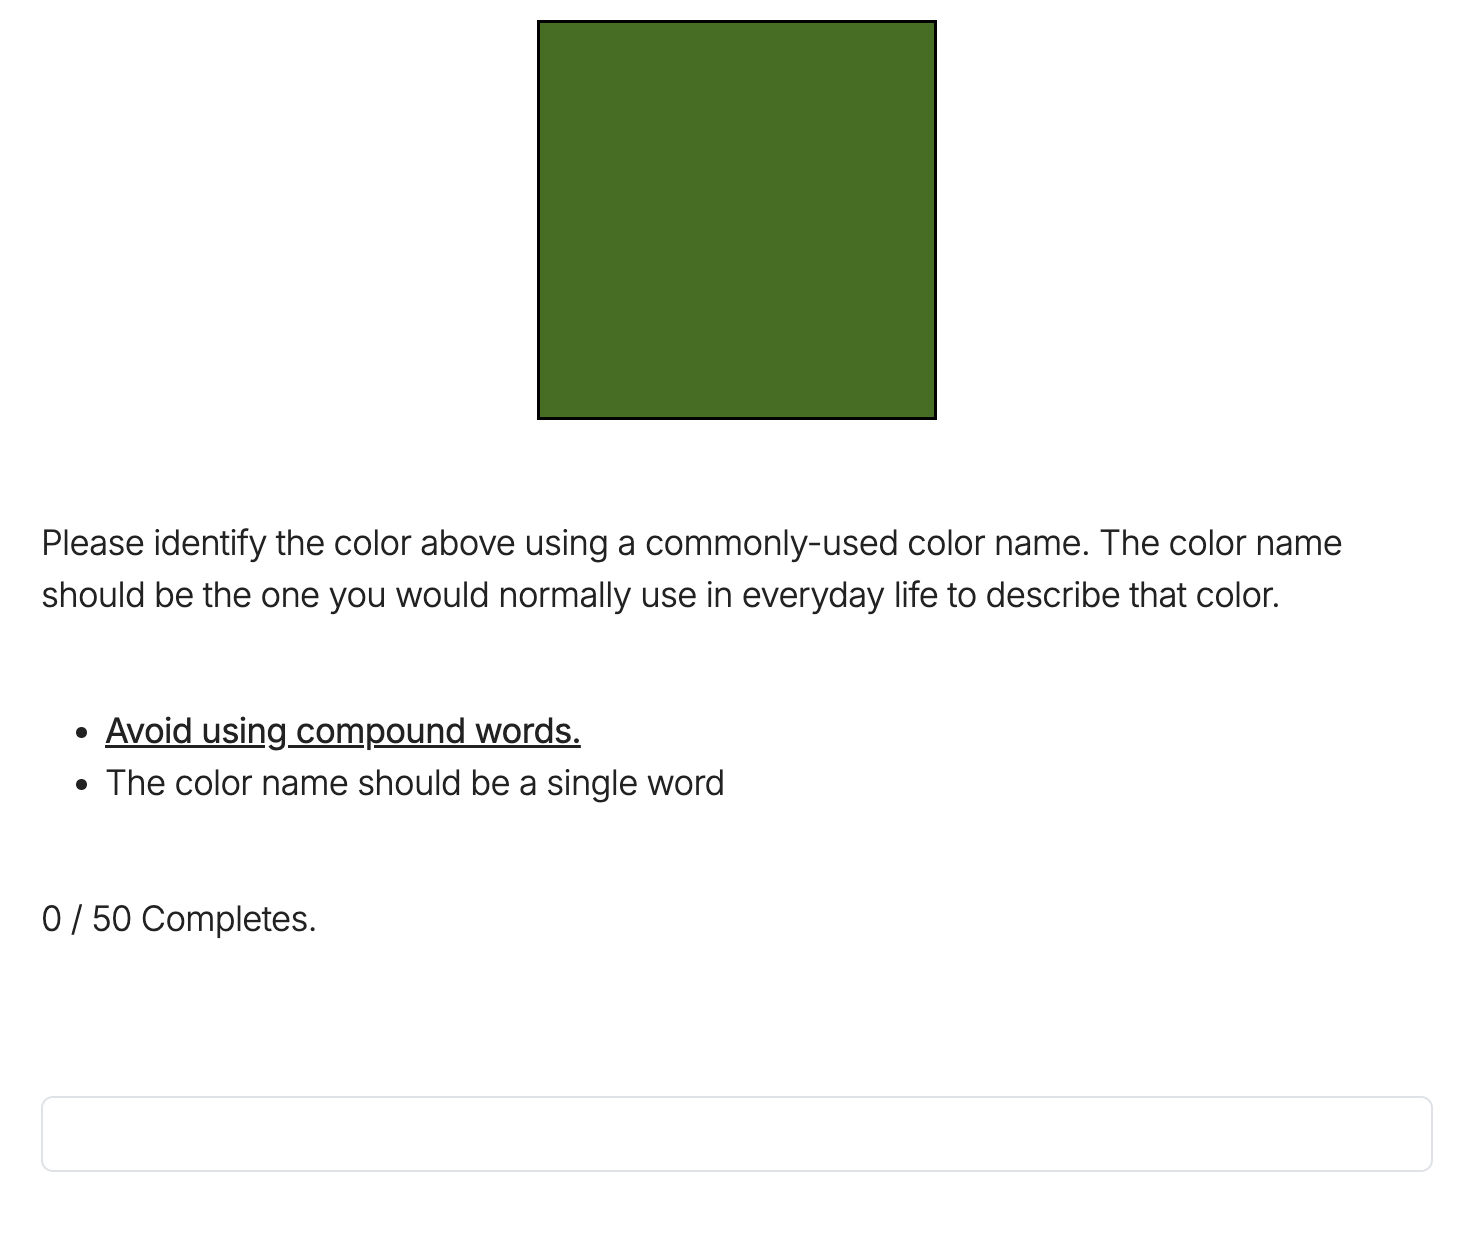
\includegraphics[width=\textwidth]{images/Color-Trail.png}}
    \decoRule
    \caption[Color trail]{Main task of the experiment, presents a square of color to the participant and requests the participant to name the color. The input had to fulfill the following requirements: Min and max number of characters obtained from data elicited from GPT4, only in the language commonly used scripts allowed, no digits, no spaces.}
    \label{fig:col-trail}
\end{figure}


The prompt was then translated by professional translators recruited with the online service translated \parencite{translated} to all 25 languages (Fig. \ref{fig:deployment_map}). Translated was fully paid by the service for their translation service.
%Overall, we collected 121,108 naming responses from the participants.


\subsection{Stimuli}
\label{stimuli}
To ensure comparability with the literature we adopted to the concept of subdividing the color space into 330 color chips \parencite{kayWorld2009}. Color space was divided into eight levels of lightness and 40 equal steps on the hue scale. This collection was complemented by 10 achromatic Musell chips ranging from black over gray to white (Fig. \ref{fig:mode_prop_maps} upper panel).
% (Fig. \ref{fig:munsell-chips}).

For the representation of colors we used the RGB color space which is based on the idea of trichromatic vision. The human eye has three types of cone photoreceptores that are most sensitive to different ranges of wavelengths. Short, Medium, and Long. These correspond roughly to the blue, green, and red parts of the spectrum, respectively. In the brain the impression of all shades of colors gets constructed through the relative excitation of these three types of cones. In digital image processing this fact is used to display every shade of each color by mixing the amount of red, green or blue for every pixel \parencite{rgb-model}.


% \begin{figure}[htp]
%     \centering
%     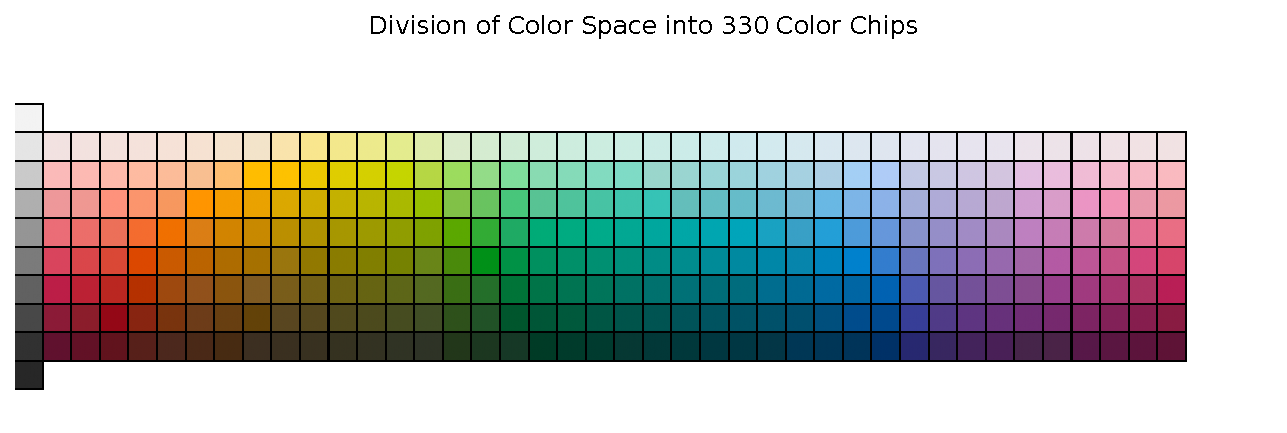
\includegraphics[width=\textwidth]{images/munsell_chips.pdf}
%     \decoRule
%     \caption[330 Munsell-Chips]{330 Munsell-Chips: Color space equally divided along hue and lightness axis (40x8).}
%     \label{fig:munsell-chips}
% \end{figure}

\begin{figure}[h!t]
\centering
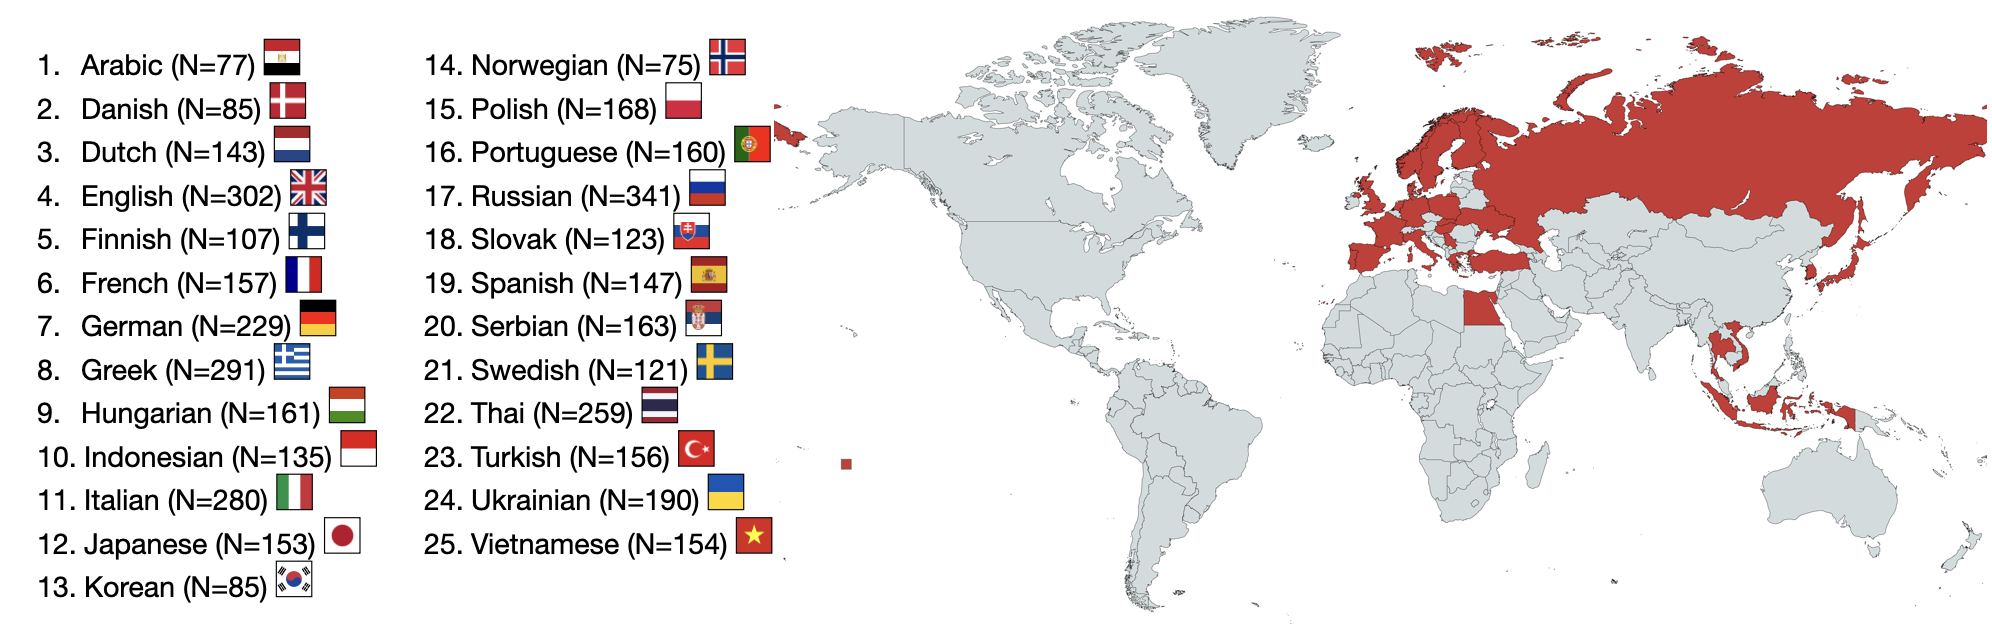
\includegraphics[page=1, width=\linewidth]{images/deployment_map.png}
\decoRule
\caption[Deployment Map]{Deployment Map: Regions in the world we recruited participants from.}
\label{fig:deployment_map}
\end{figure}


\section{Participants}
\label{sec:participants}
All participants provided informed consent according to an approved protocol (Max Planck Ethics Council \#2021\_42) and were recruited through Prolific \parencite{prolific} and Lucid Marketplace \parencite{lucid}.
Data were collected from 29 groups (25 in Lucid and 4 in Prolific, with 25 unique languages, see Figure \ref{fig:deployment_map}). 
Per group between 75 and 259 participants were recruited (mean: 150.0, sd=39.6). We aim to recruit about 160 people per group and at least 75 per group. The number of participants was matched to previous literature and our pilot data. Importantly, the difficulty (time to recruit) was different across locations. This resulted that the number of participant varied from location to location. We recruited the data in two batches: one in Summer 2023 (from 13/06/2023 - 10/8/2023) and one in early 2024 (from 11/03/2024 - 15/03/2024). 
Altogether, we collected data from 4,351 participants (Lucid: 3,834, Prolific: 517).
The mean age across all participants was 42 (sd=15) and the male to female ratio was 38.5 \% female. Participants had in average 1.5 (sd=3.6) years of formal training and 2.0 (sd=6.2) years of non formal training in the field of color related activities. 
For all languages the wikivocab score was very high, in average 80\% right answers.
The wage per hour was adapted to the local minimal wage.  Summary information about all recruited groups can be found in Table \ref{tab:pgfplotstable_csv}.


\begin{sidewaystable}[htp]
\centering
\resizebox{0.9\textwidth}{!}{%
    \pgfplotstabletypeset[
        col sep=comma,
        string type,
        every head row/.style={before row=\hline, after row=\hline},
        every last row/.style={before row=\hline\hline, after row=\hline},
        every first column/.style={column type=|l},
        every last column/.style={column type=l|},
    ]{images/participants_table.csv}
}
\caption{Participants}
\label{tab:pgfplotstable_csv}
\end{sidewaystable}


% HERE YOU MAY WANT TO PROVIDE INFORMATION ON THE GPT EXPERIMENTS BECAUSE DATA CLEANING IS UNCLEAR IF YOU DON"T KNOW ABOU THESE EXPERIMENTS.
\section{GPT4 data collection}
In a second experiment participants were replaced with a LLM.
Here data collection was done by Dr. Ilia Sucholutsky analogous to the elicitation of the human data. As an LLM, OpenAI's GPT4 \parencite{achiam2023gpt} was examined using the Microsoft Azure OpenAI API (version 0613 of the model).
Data collection was performed with the default value of the hyperparameter temperature = 0.7.
Consolidating GPT4 via the API enables two steps of prompting. The system prompt is used to prepare the model for the experiment: ``Follow all instructions that users provide to you in their own language. Respond to users in their own language using only a single word and no other text. Do not use any compound words.''
For each languages we then used the exact same elicitation prompt we used for humans translated into the respective language. For GPT4 instead of showing the visual color we specified the colors as hexcodes: 

``COLOR: $<$hexcode$>$
Please identify the color above using a commonly-used color name. The color name should be the one you would normally use in everyday life to describe that color. Avoid using compound words. The color name should be a single word.'' 
50 responses per color chip for each language were collected.

The LLM-V dataset was obtained through the utilization of OpenAI's GPT4-V (version GPT4-vision-preview, accessed via Microsoft Azure's OpenAI API), employing a methodology consistent with the one previously delineated. However, instead of providing GPT4 with a hexadecimal code, the process involved the presentation of a Base64 encoded image representative of the specific color.


\section{Data Cleaning}
The paradigm used in this study elicited free text. Therefore, we had to clean these results in several steps. The main problems appeared to be invalid answers, inconsistent use of grammatical forms, diacritics, special scripts, compound words and typos. The data cleaning was done in the same manner for humans and GPT4 data.


\subsection{Exclusion of invalid answers}
The first step in the cleaning pipeline was to exclude invalid answers such as "Error", "Nan", empty answers, answers containing spaces, digits, punctuation, only capital letters as we assumed them to be acronyms, or if scripts were used which are not common in the respective language. This can also occur when GPT4 and human did not provide valid responses and thus this "empty" response needs to be eliminated from further processing.
Exclusion of unusual scripts was done by first identifying the Unicode blocks\footnote{\url{http://unicode.org/Public/UNIDATA/Blocks.txt}} of the responses and then counter check if these are present in a list of scripts we specified beforehand.

\subsection{Lemmatization}
For languages under support (excluding Arabic Japanese, Serbian, Thai and Vietnamese), we applied lemmatization \parencite{jurafskySpeech}\footnote{\url{https://pypi.org/project/simplemma/}} . In order to group the same words together, different forms of the same term get "reduced" to its root or lemma. This is more elegant than other methods, such as stemming.

\subsection{Diacritics}
Some languages include the use of diacritics in their alphabet.
However, the participants did not use these diacritics consistently. 
To match the versions of each color term with and without diacritics, we removed them and then replaced all occurrences with the most common version. 
This was done using the python unicodedata library \footnote{\url{https://docs.python.org/3/library/unicodedata.html}}.
Arabic is a special case where pronunciation has an impact on the written form of a letter, including diacritics. Therefore, different dialects can lead to modified writing and characters \parencite{owens2013oxford}. A list of letters were identified that are most exposed to this influence and unified across the dataset (\textarabic{ى, ؤ, إ, أ, ئ, ة} to \textarabic{ي, و, ا, ا, ي, ه}).


\subsection{Special scripts}
We regarded Japanese and Korean as employing "special scripts." 
Japanese incorporates three distinct scripts in its writing system: Kanji, which is logographic, and two syllabic scripts, Hiragana and Katakana\parencite{harai2007japanese}.
Participants seem not to use a single script exclusively.
To universalize the scripts, we transformed all answers into katakana using the pykakasi\footnote{\url{https://pypi.org/project/pykakasi/}} package.
The most common script in Korean is Hangul where single syllables are put together in blocks \parencite{pae2018korean}.
To decomposed different writings of the same words we syllabified all answers into their Jamos or components. We used for this purpose the jamotools\footnote{\url{https://pypi.org/project/jamotools/}} python package.
%This was done using the "jamotools" python package.

\subsection{Compound words}
To remove compound words we identified frequent color terms (occurring in >1\% of answers).
For all these words we iterated over all unique color terms and checked weather they end with that word. If this was the case and the two terms co occurred in the dataset we replaced the compound word with the base (e.g. "hellblau" -> "blau").
This heuristic assumes that in case of color terms compound words are built from a base which is the main color category referred to and a modulator part placed beforehand giving it a specified shade.
This was however not applicable to Arabic.

\subsection{Typos}
Typos were detected based on the frequency of a word in the respective language calculated using "thefuzz" library \footnote{\url{https://pypi.org/project/thefuzz/}}. If the score exceeds the threshold of 80 the color term was replaced with the most similar color term which was evaluated using the Levenstein edit distance and co-occurrence in the dataset.

\subsection{Rare words}
As a last cleaning step infrequent color terms (occurring in less than 1\% of all answers) where deleted from the dataset even if the exclusion of these color terms lead to the extinction of all answers for a color chip so that no data were left to name this color chip. If this was the case instead of deleting these color terms from the data they were mapped to one of the frequently used color terms they most co-occurred with in the data. 